\newpage
\subsection{Participating media}
\label{sec:media}
\vspace{-1cm}
\renderings{
	\subfloat[A knitted sheep sweater (Ridged Feather pattern)]{
	\fbox{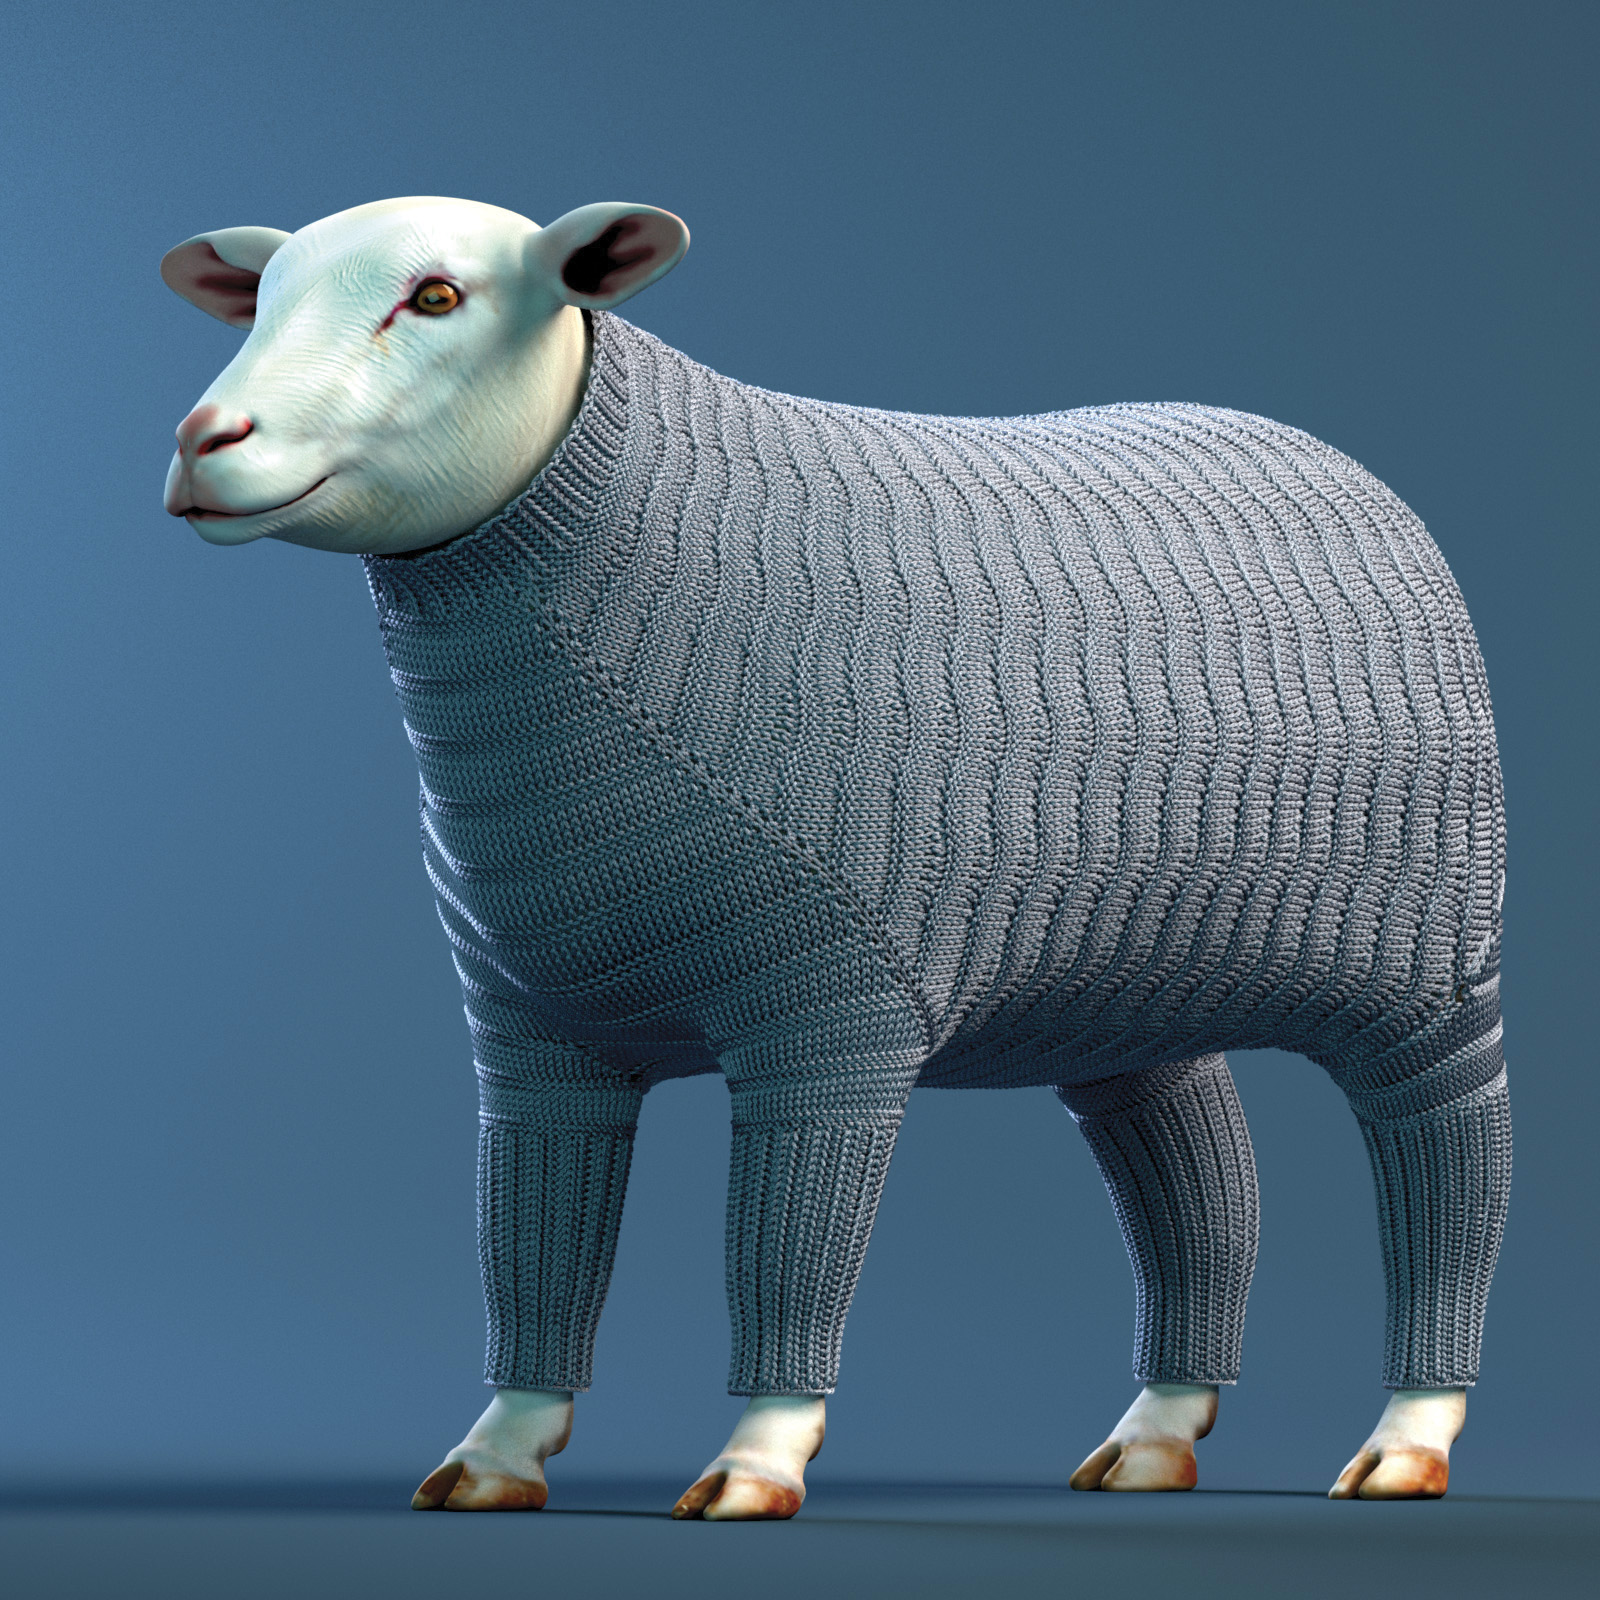
\includegraphics[width=0.58\textwidth]{images/medium_sheep}}}\hfill
	\subfloat[A knitted sweater for an alien character (Braid Cables pattern)]{
	\fbox{
\includegraphics[width=0.32\textwidth]{images/medium_alien_cables}}}\hfill
	\vspace{-2mm}
	\caption{Participating media are not limited to smoke or fog: they are
	also great for rendering fuzzy materials such as these knitted sweaters
	(made using the \pluginref{heterogeneous} and \pluginref{microflake} plugins).
	Figure courtesy of Yuksel et al. \cite{Yuksel2012Stitch}, models courtesy of
	Rune Spaans and Christer Sveen.}
}
In Mitsuba, participating media are used to simulate materials ranging from
fog, smoke, and clouds, over translucent materials such as skin or milk,
to ``fuzzy'' structured substances such as woven or knitted cloth.

This section describes the two available types of media
(\pluginref{homogeneous} and \pluginref{heterogeneous}). In pratice, these
will be combined with a phase function, which are described in \secref{phase}.
Participating media are usually also attached to shapes in the scene.
How this is done is described at the beginning of \secref{shapes} on page
\pageref{sec:shapes}.

When a medium permeates a volume of space (e.g. fog) that includes sensors or emitters,
it is important to assign the medium to them. This can be done using the
referencing mechanism:

\begin{xml}
<medium type="homogeneous" id="fog">
	<!-- .... homogeneous medium parameters .... -->
</medium>

<sensor type="perspective">
	<!-- .... perspective camera parameters .... -->

	<!-- Reference the fog medium from within the sensor declaration
	     to make it aware that it is embedded inside this medium -->
	<ref id="fog"/>
</sensor>
\end{xml}
